\section{Anforderungsanalyse}
Das folgende Kapitel analysiert den bestehenden Prozess zur Ressourcenübersicht
beim \gls{HOD} Systemtest. Basierend auf dieser Analyse wird der Soll-Zustand 
des Projekts definiert, indem genaue Anforderungen an das System gestellt werden. 
Diese Anforderungen werden priorisiert, um am Ende die Funktion des 
fertigen Systems zu validieren.

\subsection{Analyse des aktuellen Testprozesses}
Aufgrund des Arbeitsverhältnisses von mehreren Jahren bei \gls{JSS} und der Entwicklung
von mehreren Programmen, die den Testprozess automatisieren oder unterstützen, ist
dem Autor dieser Arbeit der Prozess äußerst bekannt. Dennoch wurden Interviews mit den Hauptbeauftragten
der unten beschriebenen Rollen durchgeführt. Um den Prozess besser zu verstehen,
wurden UML Aktivitätsdiagramme erstellt. Da die Rollen teilweise wenig 
miteinander interagieren, wurden die Prozesse der jeweiligen Rollen einzelnen
betrachtet.\\

Der aktuelle Testprozess basiert auf einem täglich erstelltem Tagesplan 
(Siehe~\nameref{fig:tagesplan}). Dieser Tagesplan beinhaltet die Tests, welche an diesem
Tag von den \gls{Techniker}n durchgeführt werden sollen, mit den wichtigsten 
Informationen, wie zum Beispiel das Programm zur Reihenfolge der simulierten Griffe.
Da diese Liste als \gls{Jira} Auszug in Form einer \gls{PDF} oder statischer \gls{HTML} Datei zur Verfügung 
gestellt wird, kann sie keinerlei Informationen zu vorherigen oder folgenden 
Tests liefern, welche jedoch für einen effizienten Umbau benötigt werden.

Weiterhin gibt es keinerlei Informationen zu Wartungszeiten der einzelnen Ressourcen.
Diese müssen in einer separaten Ressourcenliste eingesehen werden
(Siehe~\nameref{fig:ressourcenliste}). Die Aktualisierung dieser Liste findet nur über 
das Versionskontrollsystem \gls{SVN} statt und liegt verborgen in einer Vielzahl
an Ordnern. Zusätzlich muss der Start der Benutzung der Ressource eingetragen
werden. Dadurch muss die Liste nach einer Wartung erneut angepasst werden. \\

 
Demnach ergeben sich folgende Prozesse:

\begin{figure}[H]
    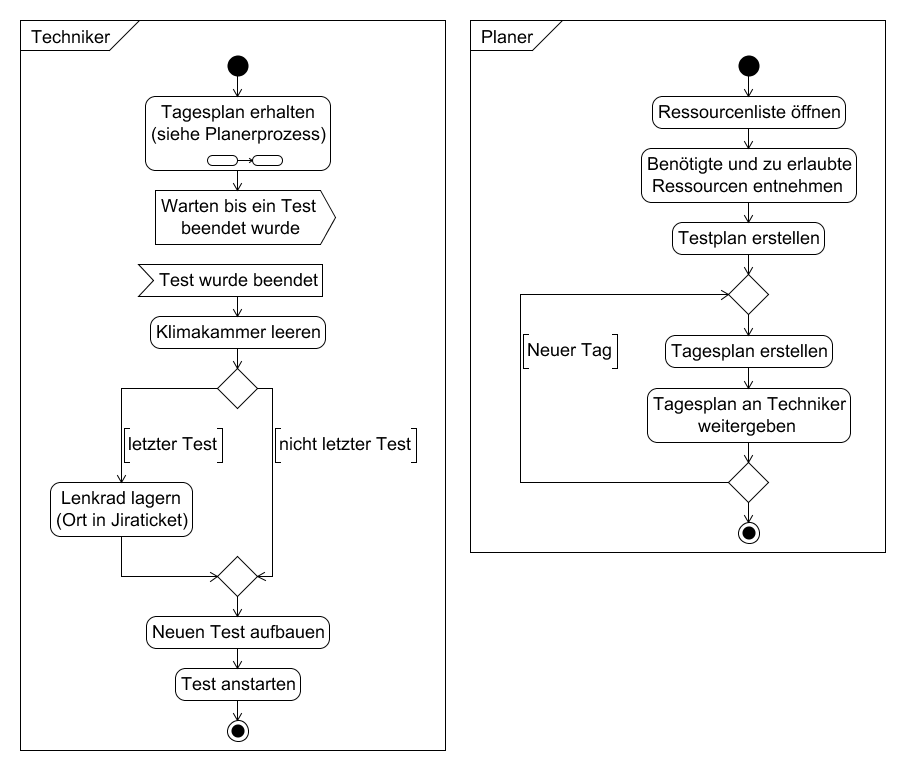
\includegraphics[width=\linewidth]{diagramme/TechnikerPlanerProzess.png}
    \caption{UML Aktivitätsdiagramm zum täglichen Testprozess}\label{fig:TechnikerPlanerProzess}
\end{figure}

Aus Abbildung~\ref{fig:TechnikerPlanerProzess} gehen zwei verschiedene Rollen hervor. Der
Planer (rechts) ist verantwortlich für das langfristige Planen von Tests. Dabei muss
dieser beachten, dass die Wartungstermine eingehalten werden, wenn
eine gewisse Ressource eingeplant wird. Welche Ressourcen zur
Verfügung stehen und wann die Wartungstermine sind, kann der Planer aus
der Ressourcenliste entnehmen. Zusätzlich erstellt der Planer auch den täglichen 
Tagesplan, welcher nur das Ergebnis eines \gls{JQL} Filters ist. 

Der Techniker (links) hingegen, ist für den Umbau und die tatsächliche Durchführung der 
Tests verantwortlich. Er benötigt den Tagesplan um zu wissen, welche Tests als 
nächstes durchgeführt werden sollen. Da im Tagesplan allerdings nicht vermerkt ist, 
welcher Test nach einem spezifischen Test durchgeführt werden muss, muss er die 
Klimakammer so weit es nötig ist leeren, um anschließend den nächsten Test 
aufzubauen. Zusätzlich weiß der Techniker nicht, welcher Test der letzte Test einer Testreihe ist.
Diese Information ist nötig, um die anschließende Lagerung des Lenkrads einzuleiten.
Um diese Information zu erhalten, muss er im jeweiligen \gls{Jira} Ticket nachschauen. \\

\begin{figure}[H]
    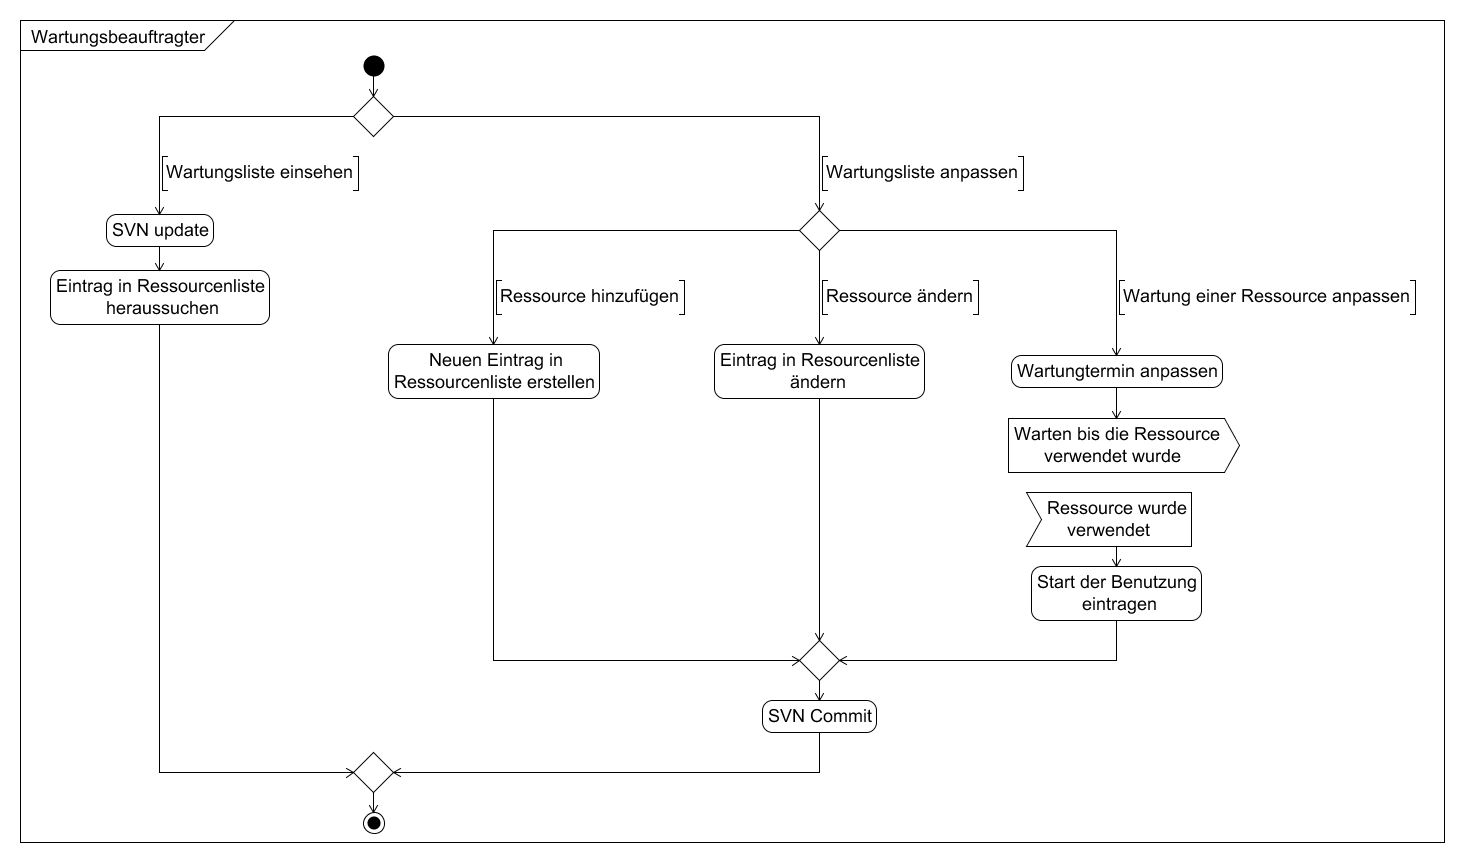
\includegraphics[width=\linewidth]{diagramme/WartungsbeauftragterProzess.png}
    \caption{UML Aktivitätsdiagramm zum Ressourcenmanagementprozess des Wartungsbeauftragten}\label{fig:WarterProzess}
\end{figure}

Der in Abbildung~\ref{fig:WarterProzess} beschriebene Prozess zeigt den Umgang mit der 
Ressourcenliste. Der Wartungsbeauftragte muss jedes mal, wenn er die Wartungsliste
einsehen will, vorher ein \gls{SVN} Update machen, um auch tatsächlich die aktuelle
Version der Liste zu erhalten. Wird dies nicht getan, kann es bei Änderungen 
zu \gls{SVN} Konflikten kommen oder die entnommenen Informationen sind veraltet.
Falls er irgendetwas an der Liste anpasst, muss diese anschließend wieder ins 
\gls{SVN} hochgeladen werden, um die Informationen mit allen anderen Mitarbeitern
zu synchronisieren. Zusätzlich muss zu jedem neuen Wartungstermin, das tatsächliche
Datum der ersten Benutzung seit der Wartung eingetragen werden. \\

Aus den zuvor aufgeführten Prozessen ergeben sich folglich die nachfolgenden Rollen:

\begin{description}
    \item[\textbf{Planer}] Die Rolle der Person, die Pläne für kurzfristige oder
    langfristige Tests erstellt.

    \item[\textbf{Wartungsbeauftragter}] Die Rolle der Person, die Wartungen 
    überwacht, plant und durchführt. 

    \item[\textbf{Techniker}] Die Rolle der Person, die Tests aufbaut, umbaut und
    durchführt.
\end{description}

Auch wenn es sein kann, dass eine Person mehrere Rollen annimmt, ist es dennoch 
wichtig die Rollen voneinander zu unterscheiden, um den Prozess nachvollziehbarer
und übersichtlicher zu gestalten.

\subsection{Einbindung in vorhandene Programme}
Da gerade die Wartungsinformationen auch in anderen Programmen benötigt werden, 
beispielsweise um Warnungen bei bald ablaufenden Wartungen bei der Testvorbereitung
anzeigen lassen zu können, ergibt sich eine weitere Rolle:

\begin{description}
    \item[\textbf{Entwickler}] Die Rolle der Person, die die Informationen der
    offenen Schnittstelle für eigene Programme verwendet
\end{description}

\subsection{Use Cases}\label{sec:usecases}
In Abbildung~\ref{fig:usecases} und Abbildung~\ref{fig:usecasesEntwickler} sind 
die bereits definierten Rollen als Akteure dargestellt.
Die Use Cases ergeben sich aus den Interviews und der Prozessanalyse.

\begin{figure}[H]
    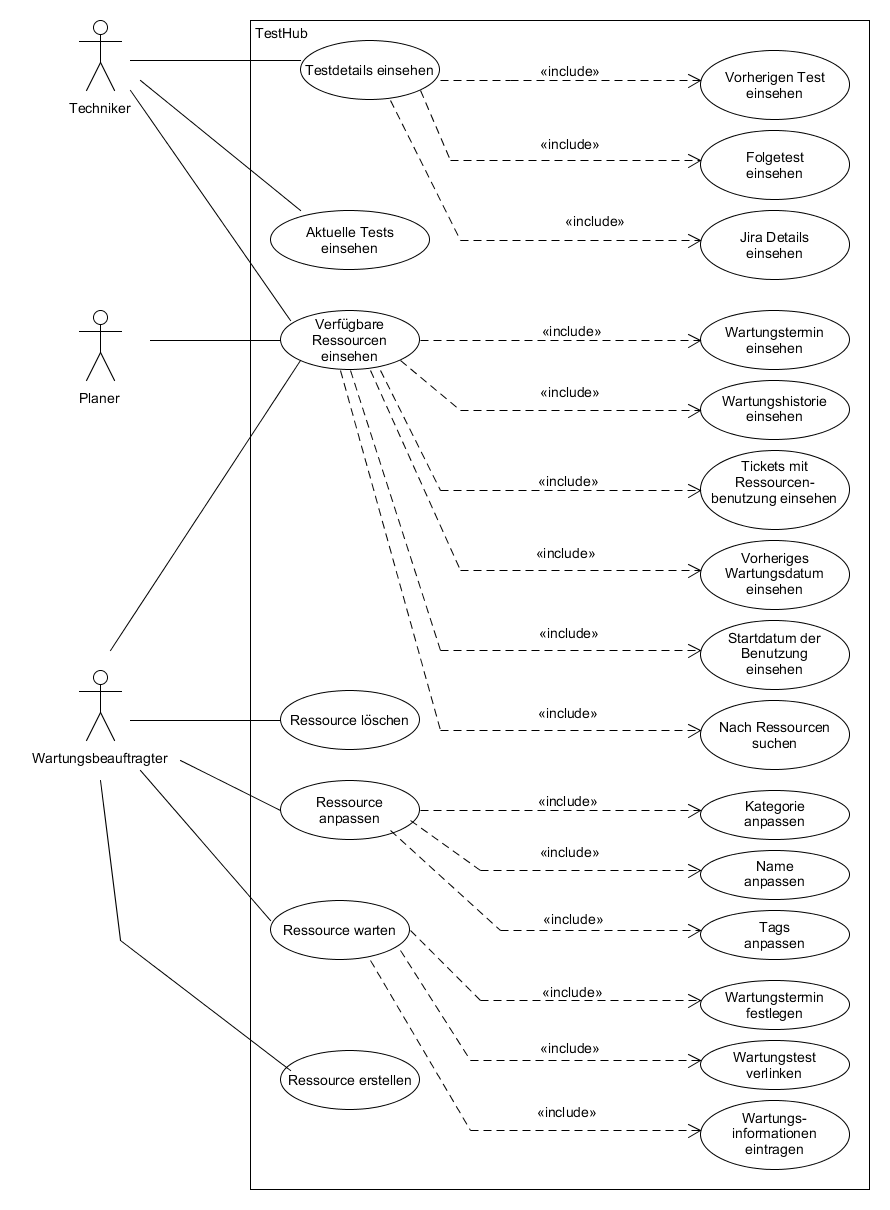
\includegraphics[width=\linewidth]{diagramme/Usecases.png}
    \caption{UML-Use-Case-Diagramm zu den Anwendungsfällen für die Planer-, Techniker- und Wartungsbeauftragten-Rolle}\label{fig:usecases}
\end{figure}

\begin{figure}[H]
    \includegraphics[width=\linewidth]{diagramme/UsecasesEntwickler.png}
    \caption{UML-Use-Case-Diagramm zu den Anwendungsfällen für die Entwickler-Rolle}\label{fig:usecasesEntwickler}
\end{figure}

\subsection{User Stories}\label{sec:userstories}
Die folgenden User Stories ergeben sich aus den zuvor definierten Use Cases.

\begin{description}
    \descitem{US\#01}{itm:us01}
    \textit{Als Techniker möchte ich einen vorherigen Test einsehen}

    \descitem{US\#02}{itm:us02}
    \textit{Als Techniker möchte ich einen folgenden Test einsehen}

    \descitem{US\#03}{itm:us03}
    \textit{Als Techniker möchte ich die Details eines Jira-Tickets in 
    aufgeschlüsselter Form einsehen}

    \descitem{US\#04}{itm:us04}
    \textit{Als Techniker möchte ich alle aktiven Tests einsehen}

    \descitem{US\#05}{itm:us05}
    \textit{Als Techniker möchte ich eine schnelle Übersicht über die wichtigsten
    Ressourcen erhalten, um den Aufbau von Tests zu planen}

    \descitem{US\#10}{itm:us10}
    \textit{Als Planer möchte ich einen Wartungstermin einsehen, um zu erfahren
    ob ich diese Ressource einplanen kann}

    \descitem{US\#11}{itm:us11}
    \textit{Als Planer möchte ich eine Wartungshistorie einsehen, um eventuelle
    vergangene Probleme aufzudecken}

    \descitem{US\#12}{itm:us12}
    \textit{Als Planer möchte ich alle aktiven Tickets sehen, 
    welche eine spezifische Ressource verwenden}

    \descitem{US\#13}{itm:us13}
    \textit{Als Planer möchte ich das vorherige Wartungsdatum einsehen, 
    um zu wissen, ob das Startdatum der Benutzung hinter dem Wartungsdatum liegt
    und ich somit die Ressource verwenden kann}

    \descitem{US\#14}{itm:us14}
    \textit{Als Planer möchte ich das Startdatum der Benutzung einsehen,
    um zu wissen, ob das Startdatum der Benutzung hinter dem Wartungsdatum liegt
    und ich somit die Ressource verwenden kann }

    \descitem{US\#15}{itm:us15}
    \textit{Als Planer möchte ich nach Ressourcen suchen}

    \descitem{US\#20}{itm:us20}
    \textit{Als Wartungsbeauftragter möchte ich eine Ressource löschen}

    \descitem{US\#21}{itm:us21}
    \textit{Als Wartungsbeauftragter möchte ich die Kategorie einer Ressource anpassen}

    \descitem{US\#22}{itm:us22}
    \textit{Als Wartungsbeauftragter möchte ich den Namen einer Ressource anpassen}

    \descitem{US\#23}{itm:us23}
    \textit{Als Wartungsbeauftragter möchte ich die Tags einer Ressource anpassen,
    um Besonderheiten oder Gruppierungen hervorzuheben}

    \descitem{US\#24}{itm:us24}
    \textit{Als Wartungsbeauftragter möchte ich einen neuen Wartungstermin festlegen}

    \descitem{US\#25}{itm:us25}
    \textit{Als Wartungsbeauftragter möchte ich das Ergebnis eines Wartungstest verlinken}

    \descitem{US\#26}{itm:us26}
    \textit{Als Wartungsbeauftragter möchte ich Informationen zu einer Wartung speichern}

    \descitem{US\#27}{itm:us27}
    \textit{Als Wartungsbeauftragter möchte ich eine Ressource erstellen}

    \descitem{US\#90}{itm:us90}
    \textit{Als Entwickler möchte ich die REST API verwenden, um die
    Informationen von ``TestHub'' in meine Programm einzubinden}

    \descitem{US\#91}{itm:us91}
    \textit{Als Entwickler möchte ich die Dokumentation
    der API ansehen, um zu verstehen wie ich die API benutzen kann}

\end{description}

\subsection{Funktionale Anforderungen}\label{sec:fas}
Um die Funktionen der im Umfang dieser Arbeit entwickelten Software validieren zu
können, müssen Anforderungen definiert werden. Diese Funktionalen Anforderungen
werden in drei Kategorien eingeteilt:

\begin{description}
    \item[\textbf{Muss-Kriterien}]Die Kriterien die ``TestHub'' als \gls{MVP} zwingend erfüllen muss

    \item[\textbf{Soll-Kriterien}]Die Kriterien die für die Funktionalität von ``TestHub''
    nicht zwingend notwendig sind, aber dennoch implementiert werden sollten.

    \item[\textbf{Kann-Kriterien}]Die Kriterien, die rein optional sind. Da es sich
    bei ``TestHub'' um ein \gls{MVP} handelt, werden diese Kriterien nicht berücksichtigt.

\end{description}

Die folgenden Anforderungen ergeben sich aus den \nameref{sec:userstories} und den
in Abschnitt~\ref{sec:usecases} aufgezeigten Use Cases. Zusätzlich ergeben sich einige 
Anforderungen aus den mit den Mitarbeitern durchgeführten Interviews:

\begin{description}

% Muss Kriterien

    \descitem{FA\#01}{itm:fa01}
    \textit{TestHub muss alle aktiven Tests nach Klimakammer gruppiert anzeigen (\descref{US\#04}{itm:us04}).}\\
    Ein Test gilt als aktiv, wenn der Status seines Jira-Tickets ``Read for Test''
    oder ``In Execution'' ist.

    \descitem{FA\#02}{itm:fa02}
    \textit{TestHub muss die Informationen eines Jira-Tickets in übersichtlicher 
    Form anzeigen (\descref{US\#03}{itm:us03}).}

    \descitem{FA\#03}{itm:fa03}
    \textit{TestHub muss die Labels eines Jira-Tickets kategorisiert anzeigen (\descref{US\#03}{itm:us03}).}\\
    Die Labels eines Jira-Tickets liegen als simple Liste von Text vor. Dieser 
    Text soll analysiert und entsprechend kategorisiert werden, um eine genauere 
    Zuordnung zu ermöglichen.

    \descitem{FA\#04}{itm:fa04}
    \textit{TestHub muss den vorherigen und folgenden Test eines aktuell 
    ausgeführten Tests anzeigen können (\descref{US\#01}{itm:us01} \& \descref{US\#02}{itm:us02}).}\\
    Ein Test kann vorherige und folgende Tests haben, es gibt jedoch auch Tests,
    bei denen dies nicht der Fall ist.    

    \descitem{FA\#05}{itm:fa05}
    \textit{TestHub muss eine schnelle Übersicht über die wichtigsten Ressourcen anzeigen (\descref{US\#05}{itm:us05}).}\\
    Die wichtigsten Ressourcen sind: aktive Tests und Ressourcen mit einem Wartungstermin
    in den nächsten 30 Tagen.

    \descitem{FA\#06}{itm:fa06}
    \textit{TestHub muss den nächsten Wartungstermin einer Ressource anzeigen (\descref{US\#10}{itm:us10}).}
    
    \descitem{FA\#07}{itm:fa07}
    \textit{TestHub muss das löschen einer Ressource unterstützen (\descref{US\#20}{itm:us20}).}
       
    \descitem{FA\#08}{itm:fa08}
    \textit{TestHub muss das Anpassen der Kategorie einer Ressource unterstützen 
    (\descref{US\#21}{itm:us21}).}

    \descitem{FA\#09}{itm:fa09}
    \textit{TestHub muss das Anpassen des Namens einer Ressource unterstützen 
    (\descref{US\#22}{itm:us22}).}

    \descitem{FA\#10}{itm:fa10}
    \textit{TestHub muss das Anpassen der Tags einer Ressource unterstützen 
    (\descref{US\#23}{itm:us23}).}

    \descitem{FA\#11}{itm:fa11}
    \textit{TestHub muss Festlegen eines neuen Wartungstermins unterstützen 
    (\descref{US\#24}{itm:us24}).}

    \descitem{FA\#12}{itm:fa12}
    \textit{TestHub muss das Erstellen einer Ressource unterstützen 
    (\descref{US\#23}{itm:us23}).}\\
    Die Ressource benötigt mindestens einen Namen und eine Kategorie und sie muss nicht zwangsläufig 
    einen Wartungstermin haben.

    \descitem{FA\#13}{itm:fa13}
    \textit{TestHub muss unabhängig von den \gls{Jira} Benutzerrechten für das HOD Projekt funktionieren}\\
    Da das System eine schnelle Übersicht schaffen soll und auch keine Möglichkeit
    bietet, \gls{Jira} Daten anzupassen, soll das System die \gls{Jira} Informationen unabhängig der \gls{Jira} Rechte anzeigen.
    Dies ergab sich auch den Interviews mit den Mitarbeitern.


% Soll Kriterien

    \descitem{FA\#20}{itm:fa20}
    \textit{TestHub soll die Suche nach Ressourcen unterstützen (\descref{US\#15}{itm:us15}).}

    \descitem{FA\#21}{itm:fa21}
    \textit{TestHub soll die Wartungshistorie einer Ressource anzeigen (\descref{US\#11}{itm:us11}).}\\
    Die Wartungshistorie enthält alle Änderungen des Wartungstermins.

    \descitem{FA\#22}{itm:fa22}
    \textit{TestHub soll alle aktiven Tickets anzeigen, welche eine spezifische 
    Ressource verwenden (\descref{US\#12}{itm:us12}).}

    \descitem{FA\#23}{itm:fa23}
    \textit{TestHub soll das vorherige Wartungsdatum anzeigen (\descref{US\#13}{itm:us13} \& \descref{US\#11}{itm:us11}).}
    
    \descitem{FA\#24}{itm:fa24}
    \textit{TestHub soll das Startdatum der Verwendung einer Ressource anzeigen (\descref{US\#14}{itm:us14}).}\\
    Das Startdatum ist das Datum des Jira-Tickets welches nach dem Wartungstermin 
    der Ressource aktualisiert wurde und die Ressource verwendet.

% Kann Kriterien

    \descitem{FA\#30}{itm:fa30}
    \textit{TestHub kann das Verlinken eines Wartungstests unterstützen 
    (\descref{US\#25}{itm:us25}).}

    \descitem{FA\#31}{itm:fa31}
    \textit{TestHub kann das Speichern weiterer wartungsspezifischer Informationen unterstützen 
    (\descref{US\#26}{itm:us26}).}

\end{description}

\subsection{Nicht-funktionale Anforderungen}\label{sec:nfas}
Es ergeben sich folgende nicht-funktionale Anforderungen aus den Interviews und 
den User Stories:

\begin{description}

% Soll Kriterien
    \descitem{NFA\#01}{itm:nfa01}
    \textit{Die REST API von TestHub soll innerhalb der Firma verwendbar sein (\descref{US\#90}{itm:us90}).}

    \descitem{NFA\#20}{itm:nfa20}
    \textit{Die REST API von TestHub soll dokumentiert und erklärt werden (\descref{US\#91}{itm:us91}).}\\
    Es soll eine Website oder ein Dokument geben, in dem alle Endpunkte der REST API
    aufgelistet und erklärt sind. Des Weiteren soll es Beispiele zum 
    Verständnis geben.

    \descitem{NFA\#21}{itm:nfa21}
    \textit{Das \gls{UI} von TestHub soll ein einheitliches Design haben.}

    \descitem{NFA\#22}{itm:nfa22}
    \textit{TestHub soll in englischer Sprache verfügbar sein, da dies die 
    Firmensprache von JSS ist.}

    \descitem{NFA\#23}{itm:nfa23}
    \textit{TestHub soll mindestens auf den Webbrowsern ``Chrome'' und ``Edge'' funktionieren}\\
    Diese zwei Webbrowser werden innerhalb der Firma verwendet.

% Kann Kriterien

    \descitem{NFA\#30}{itm:nfa30}
    \textit{TestHub kann die Verteilung der Jira-Tickets auf die einzelnen Projekte 
    aufzeigen (\descref{US\#05}{itm:us05}).}

    \descitem{NFA\#31}{itm:nfa31}
    \textit{TestHub kann ein Gantt-Diagramm zur besseren Übersicht von aktuellen Tests anzeigen}


    
\end{description}

\newpage